
\section{Isolation}
\label{sec:isolation}
In leading-order perturbative calculations, prompt photons are produced surrounded by small hadronic activity and fragmentation photons are only found within a jet. Beyond leading order, the direct and fragmentation components have no physical meaning and cannot be factorized; the sum of their cross sections is the physical observable. However, theoretical calculations can be simplified through the use of an isolation requirement, which also suppresses the background from decays of neutral mesons.

We construct an isolation variable using only tracking information and avoid using calorimeter clusters. This choice prevents biases due to the correlation between 
isolation criteria and $\pi^{0}$ decay opening angle and allow us to use the full acceptance of EMCal. This is at the expense of a lower purity.

The isolation variable for this analysis is defined as the scalar sum of the transverse momentum of charged particles within an angular radius around the cluster direction, $R =\sqrt{(\Delta\varphi)^{2} +(\Delta\eta)^{2}  } =0.4$ (with $\Delta\varphi$ measured in radians), thus:
\begin{equation}
\iso^{\mathrm{raw}} = \sum_{\mathrm{track}~\in~\Delta R < 0.4}  \pt^{\mathrm{track}}   
\label{eq:isoraw}
\end{equation}
The charged particles used as input for the isolation calculation have {$0.15<\pt<10$ \GeVc}, {$|\eta|<0.8$} and pass the selection described in Section~\ref{sec:tracking}. 

The isolation variable defined in Equation~\ref{eq:isoraw} is susceptible to background from the charged particles from the underlying event, e.g. a truly isolated photon might appear non isolated due to overlap with particles not associated with the hard scattering. In order to correct for this effect, we apply an event-by-event underlying event subtraction, which is described in the following section. 

\subsection{Underlying Event estimation}
\label{sec:UEsubtraction}
In this section, we describe how we estimate and subtract the ``underlying event'' (UE). The UE is defined as the particles not associated with the hard-scattering of the collision\footnote{In Ref.~\cite{ALICE:2011ac}, the UE is defined as ``the sum of all the processes that build up the final hadronic state in a collisions excluding the hardest leading order partonic interaction. This includes fragmentation of beam remnants, multi-parton interactions and initial and final-state radiation associated with each interaction."}. We subtract the UE from the measured transverse momentum of jets and in the photon isolation (described in Section~\ref{sec:isolation}). 
Technically, the discrimination between the soft component from the hard component of an event is performed using the \textsc{Fastjet} jet area/median method~\cite{Cacciari:2009dp}, which uses the median of the distribution of transverse momentum densities of all jets in an event. We use one of the standard jet areas definition implemented in \textsc{FastJet} called Voronoi area~\footnote{The method used is the following fastjet::VoronoiAreaSpec \url{http://www.fastjet.fr/repo/doxygen-2.4.5/classfastjet_1_1VoronoiAreaSpec.html} }.

The estimation of the UE density uses jets $J'$ reconstructed by the
$k_{\mathrm{T}}$-algorithm\footnote{In contrast to the anti-$k_{\mathrm{T}}$ algorithm, the $k_{\mathrm{T}}$ algorithm clusters the softest particles first, and thus is more sensitive to the details of the distribution of softer objects and better suited for an investigation of the underlying event.} with distance parameter $R=0.3$. The estimated UE
density is defined as:
\begin{equation}
  \rho = \mathrm{med} \left\{ \frac{\sum_{i\in J'_k}
    p_{T,i}}{\sum_{i\in J'_k} A_i} \right\}
\end{equation}
where $p_{T,i}$ is the transverse momentum, and $A_i$ the Voronoi area
of the particle $i$ within the jet reconstructed for UE estimation
purpose $J'_k$. Following standard practice, the two leading jets are not considered in this observable, to limit the contribution from the hard component of the interaction. 

The choice of the median is motivated by its robustness against outliers, which includes jets originated by hard interactions. The observable
thus isolates UE  by assuming that most of the event is either empty or dominated by soft contributions and that the hard component of the interaction is well contained within the leading jets~\citep{Cacciari:2009dp}. 

Figure~\ref{fig:Rho} shows the median charged-particle density, $\rho$, distribution obtained in pp and p-Pb data in minimum bias events and in events that pass the selection in Section~\ref{sec:eventselection} and thus have a high-$\pt$ cluster. The distribution in minimum-bias events decreases approximately exponentially. The distribution in photon-triggered events is different and follows sort of an asymmetric Gaussian distribution that peaks at approximately {1.0 \GeVc} and {2.5 \GeVc} for pp and \pPb~collisions, respectively. 
\begin{figure}
\center
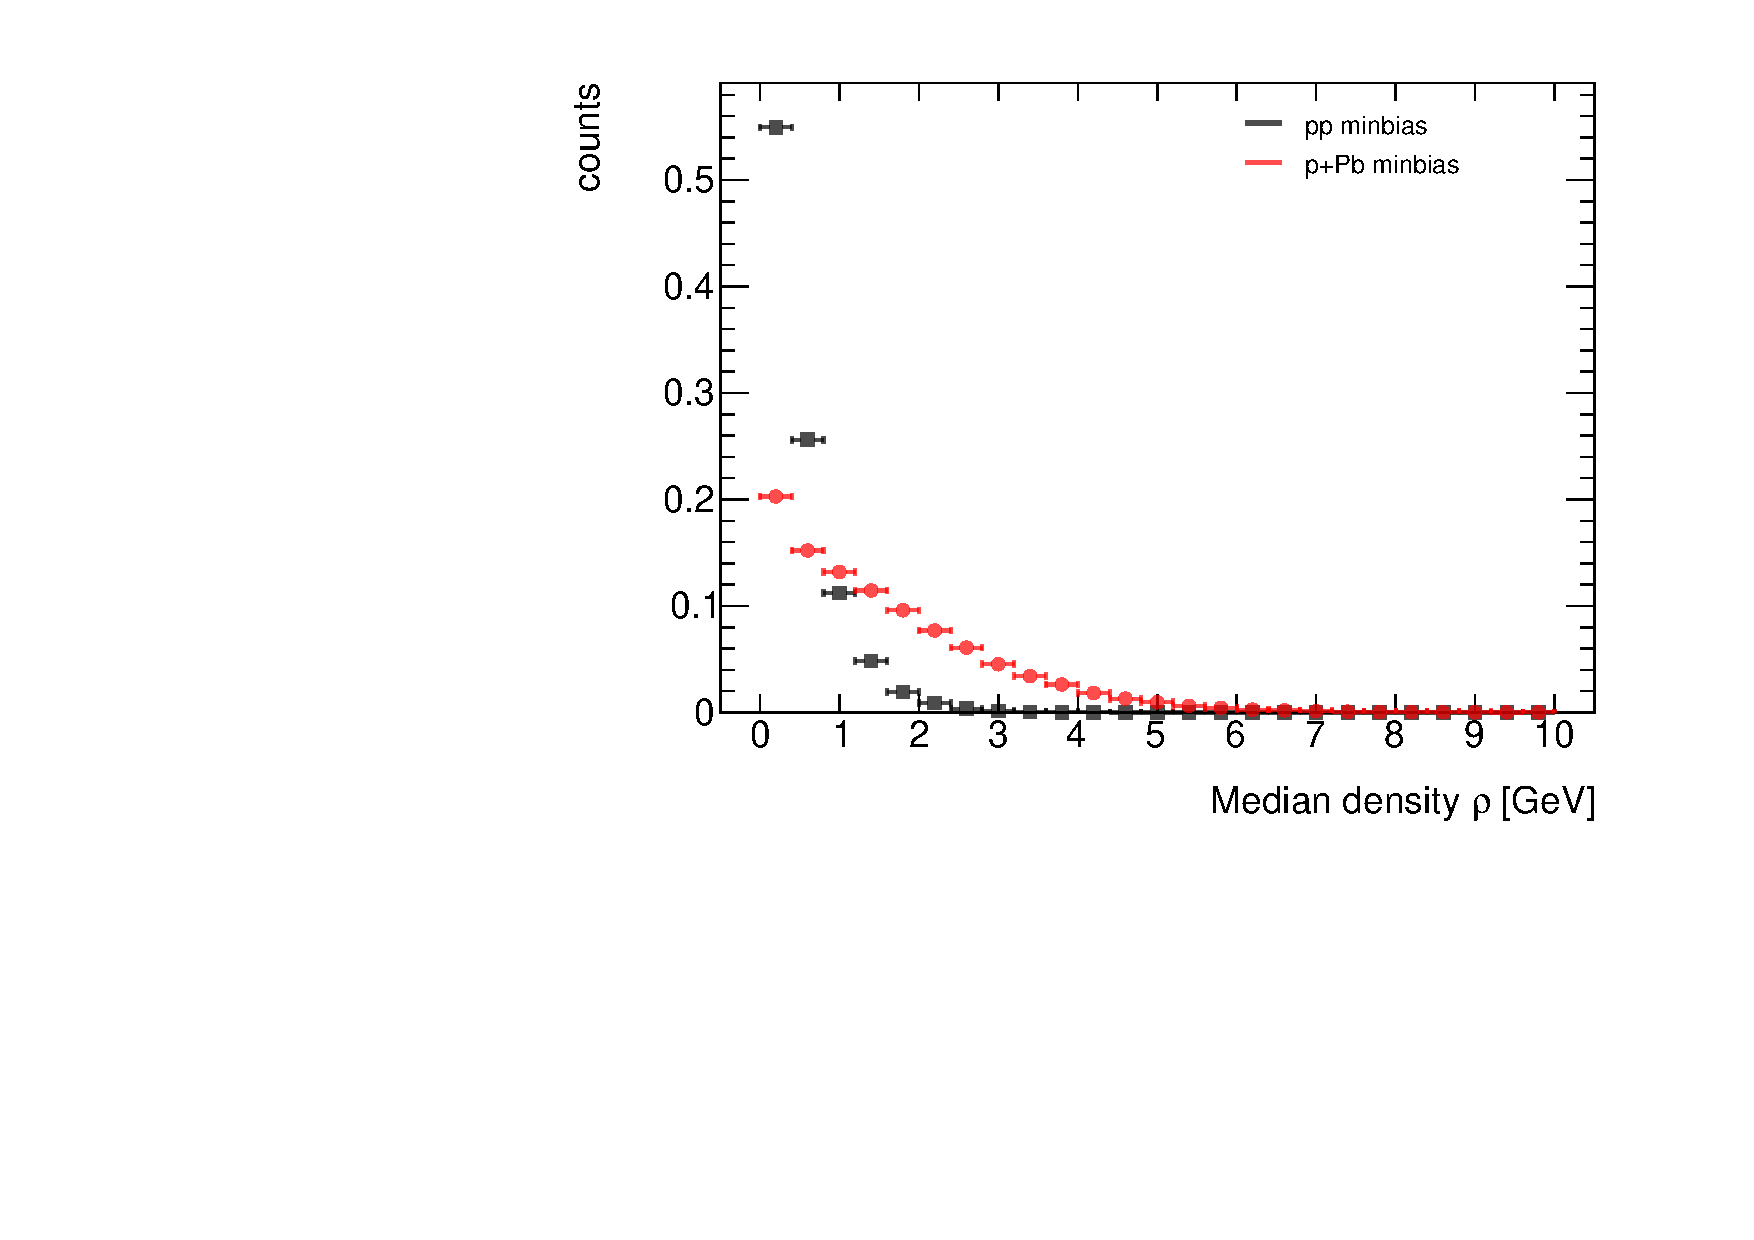
\includegraphics[width=0.49\textwidth]{UE/Rho_MinBias}
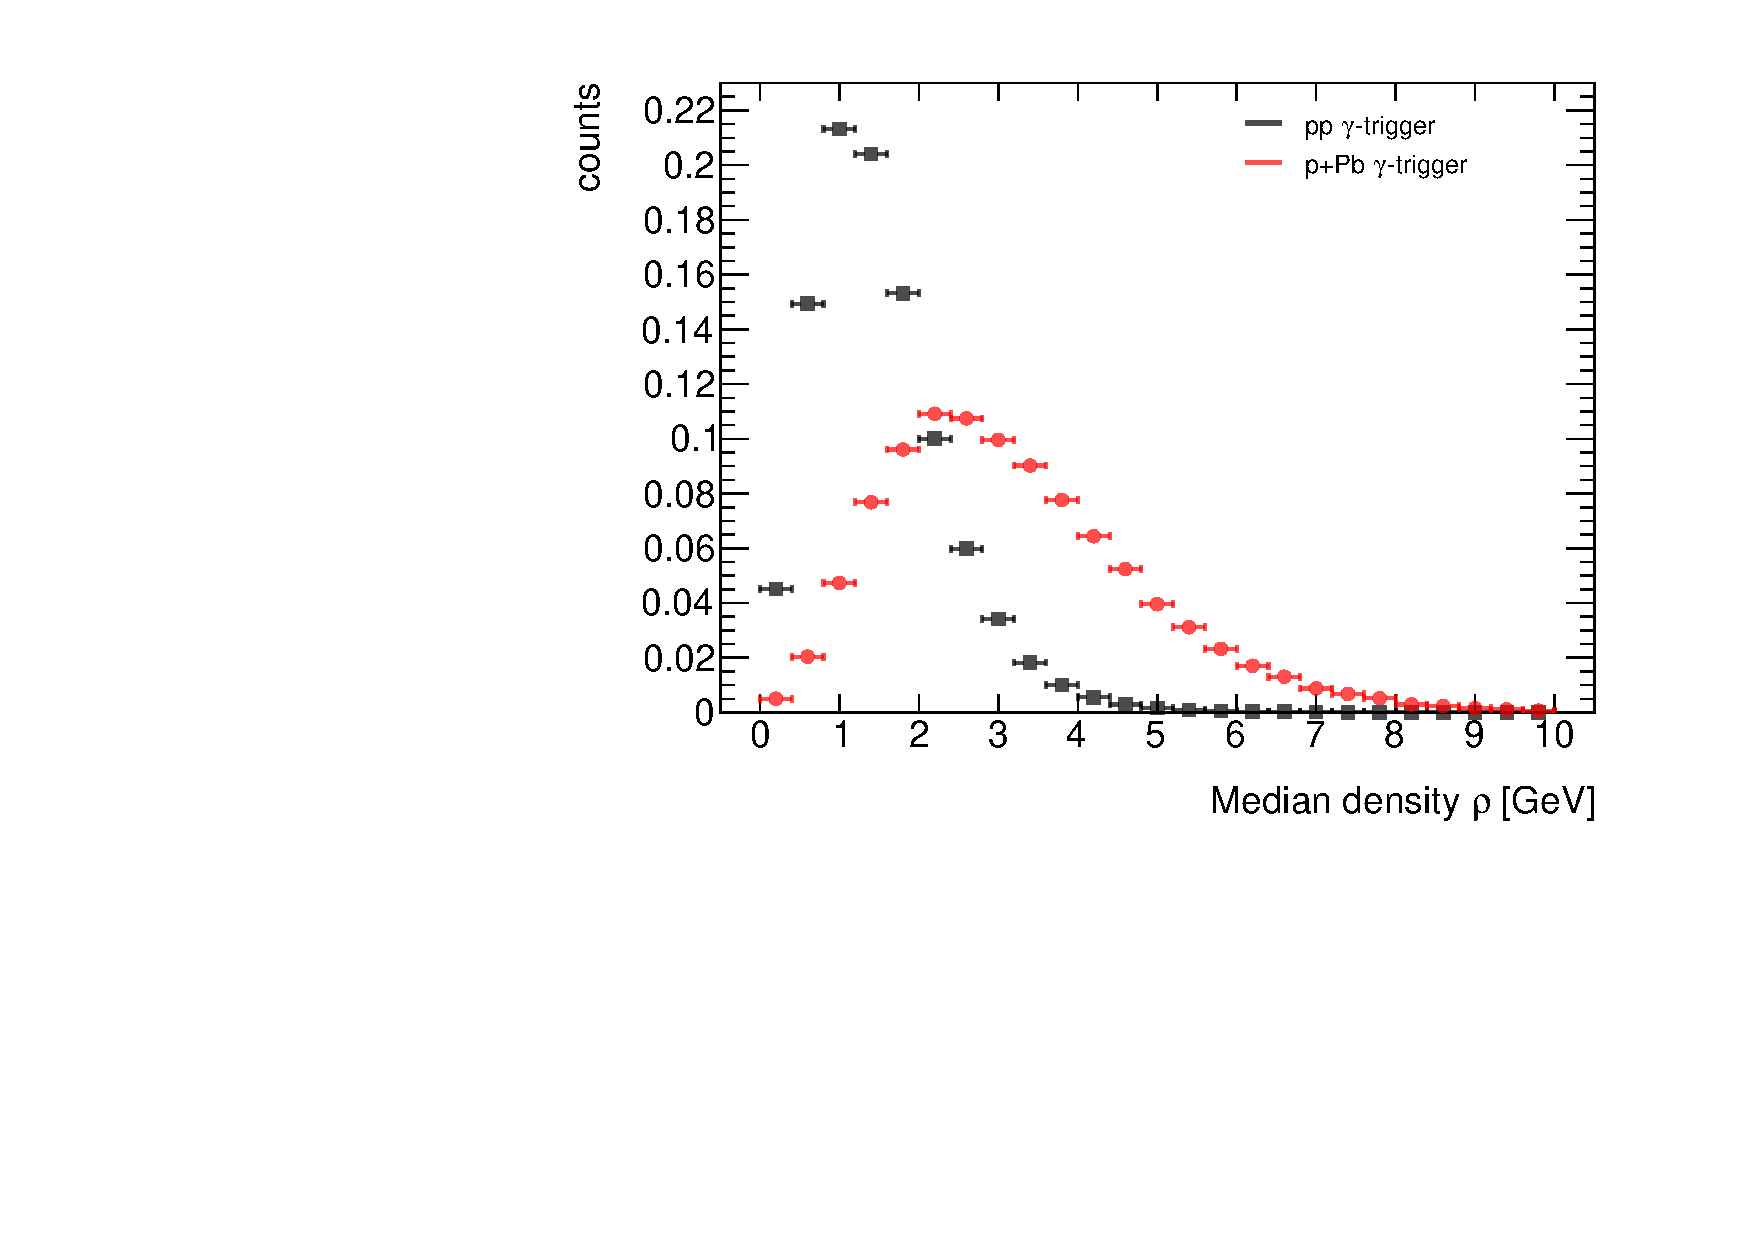
\includegraphics[width=0.49\textwidth]{UE/Rho_GammaTrigger}
\caption{Distribution of the median charged-particle transverse momentum density, $\rho$, in pp and \pPb~data, for a minimum-bias selection (left panel) and in photon-triggered events (right panel). }
\label{fig:Rho}
\end{figure}

The mean and standard deviation for each distribution is shown in Table~\ref{tab:rhoestimates}. The difference in UE-density in \pPb~is expected due to the increased number of nucleon-nucleon collisions. The UE-densities shown here are still about a factor of 50 lower than in central Pb-Pb collisions.
\begin{table}[h]
   \centering
   \caption{Median transverse momentum density mean and standard deviation in minimum-bias and and photon-triggered events in pp and \pPb~data. The statistical uncertainty in these numbers is negligible.}
   \label{tab:rhoestimates}
   \begin{tabular*}{1.0\columnwidth}{@{\extracolsep{\fill}}lcc|cc@{}}
    \hline
     &  pp minbias & pp $\gamma-$trigger & \pPb~ minbias & \pPb~$\gamma$-trigger  \\
       \hline
       $\langle\rho\rangle$   & 0.49 \GeVc & 1.51 \GeVc & 1.56 \GeVc & 3.19 \GeVc \\ 
       $\sigma_{\rho}$       &  0.47 \GeVc &  0.85 \GeVc  & 1.32 \GeVc & 1.60 \GeVc \\ 
            \hline        
   \end{tabular*}
\end{table}

The average $\rho$ for photon-triggered events reported in Table~\ref{tab:rhoestimates} is consistent with an independent estimate, based on the ``$\eta$-band'' method, that uses the same dataset and cluster selection~\cite{Erwann}. 


%\subsubsection{UE subtraction for jet transverse momentum}
%In this section, we show the result of using the measured median density to estimate UE-background for jets. We perform a jet-by-jet subtraction event-by-event. The subtracted transverse momentum of a given jet is:
%\begin{equation}
%  p_{\mathrm{T, rec}} = p_{\mathrm{T,raw}} - \rho \times A. 
%    \label{eq:jetsubtraction}
%\end{equation}
%\FloatBarrier
%Here $p_{\mathrm{T, rec}}$ is the raw transverse momentum and $A$ is the jet area.

%This approach neglects the fact that the UE-density for a given event is not uniform in $\eta$-$\phi$ but fluctuates from region to region. These fluctuations are mainly Poissonian but also encode correlated region-to-region variations of the particle multiplicity and mean $\pt$. 

%We check the impact of the fluctuations on the UE-subtraction by using Equation~\ref{eq:jetsubtraction} to measure the jet transverse momentum distribution in minimum-bias events, where the contribution from jets from a hard scattering is minimal and the reconstructed jets arise mainly from the UE and its fluctuations. That is, ideally the $p_{\mathrm{T, rec}}$ distribution should be a very narrow distribution centered around zero. 

%igure~\ref{fig:JetUE} shows the UE-subtracted transverse momentum distribution of jets in minimum-bias events in pp and p-Pb data. Only jets with $|\eta|<0.5$ are shown. In both cases, the distribution is centered around zero (the mean of the distribution if {$-$0.08 \GeVc} for pp and {0.02 \GeVc} for p-Pb data), and falls rather rapidly to both sides (the standard deviation is {1.13 \GeVc} for pp and {1.35 \GeVc} for p-Pb data). This demonstrates that the UE-subtraction for jet reconstruction works as intended. 

%\begin{figure}
%	\center
%	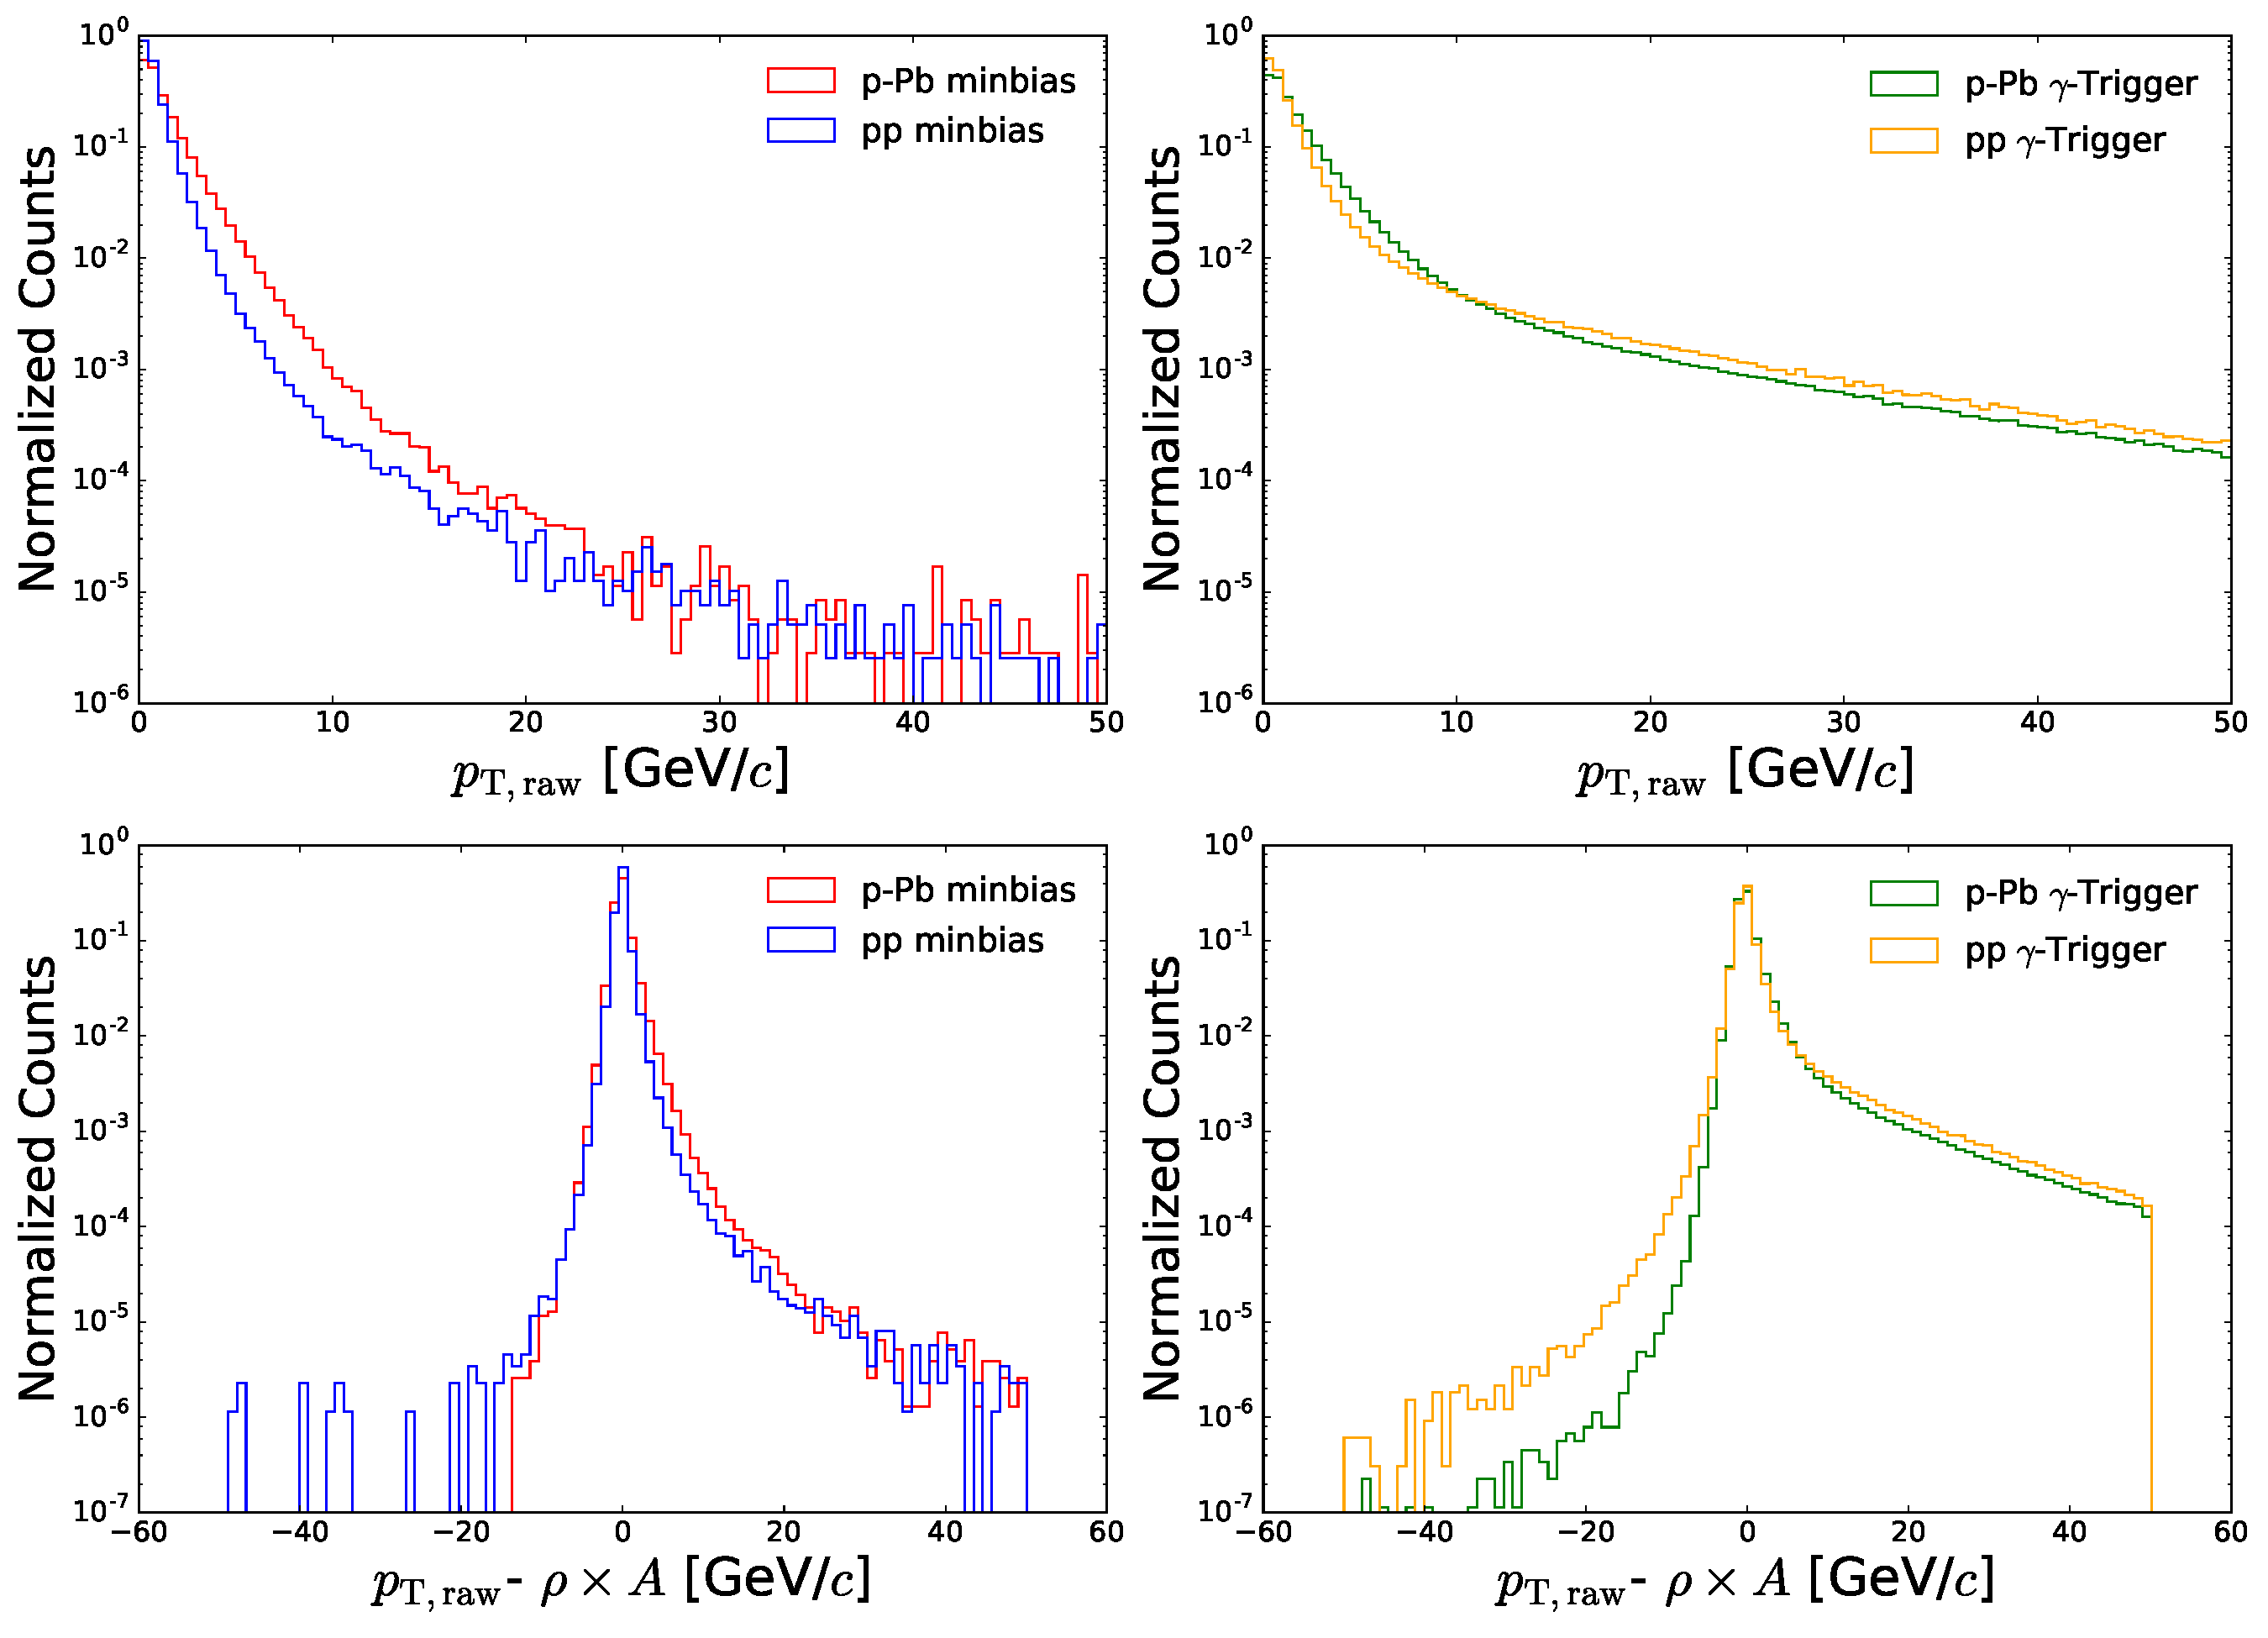
\includegraphics[width=0.9\textwidth]{UE/ppandpPb_jet_distributions.pdf}
%	\caption{A comparison between the jet transverse momentum distributions, both raw and  UE-subtracted, for minimum-bias and photon-triggered events in pp and p-Pb data. The raw jet transverse momentum distributions in minimum-bias events (upper left) and photon-triggered (upper right) in pp and p-Pb data are shown on the upper row. The UE-subtracted jet transverse momentum distributions in minimum-bias event (bottom left) and photon-triggered events (bottom right) in pp and p-Pb data are shown on the bottom row.}
%\label{fig:JetUE}
%\end{figure}

%The unphysical negative tail in Figure~\ref{fig:JetUE} arises due to UE over-subtraction. That is, the local UE density in the jet area is significantly lower than the calculated median density. On the other hand, the positive tail could be due to under-subtraction, however there are also a contribution from hard-scatterings in minimum-bias events, and there is a clear enhancement in photon-triggered events, as expected. 

%Table~\ref{TableUEUnderAndOverSubtraction} shows the fraction of jets shown in Figure~\ref{fig:JetUE} that satisfy a given threshold in subtracted  $p_{\mathrm{T, rec}}$. The results show that over-subtraction results in less than 0.5$\%$ of jets with $p_{\mathrm{T, rec}}<-3$ \GeVc. The fraction of jets with $p_{\mathrm{T, rec}}>5$ \GeVc~is less than a percent in minimum-bias p-Pb events, and drops to $0.13\%$ $p_{\mathrm{T, rec}}>10$ \GeVc. This informs our choice of minimum $p_{\mathrm{T, rec}}$ selection used for photon--jet analysis presented in Section~\ref{sec:GammaJet}. 

%\begin{table}[h]
%   \centering
%   \caption{Fraction of jets satisfying various UE-subtracted transverse momentum ranges in minimum bias events.}
%   \begin{tabular*}{1.0\columnwidth}{@{\extracolsep{\fill}}lccccc@{}}
%    \hline
%         &  pp minbias & p-Pb minbias  \\
%       \hline13

%       $p_{\mathrm{T,rec}}$ = $p_{\mathrm{T,raw}}$ - $\rho \times A$ $<$ $-$5.0 \GeVc & 0.05$\%$ & 0.05$\%$  \\ 
%       $p_{\mathrm{T,rec}}$ = $p_{\mathrm{T,raw}}$ - $\rho \times A$ $<$ $-$3.0 \GeVc & 0.32$\%$ & 0.46$\%$  \\
%       $p_{\mathrm{T,rec}}$ = $p_{\mathrm{T,raw}}$ - $\rho \times A$ $<$ $-$1.5 \GeVc & %3.24$\%$ & 5.28$\%$  \\
%       $p_{\mathrm{T,rec}}$ = $p_{\mathrm{T,raw}}$ - $\rho \times A$ $<\:\:\:\:\:\:\:\:\:\:\:$ 0 \GeVc & 63.52$\%$ & 61.55$\%$  \\
 %      \hline
 %      $p_{\mathrm{T,rec}}$ = $p_{\mathrm{T,raw}}$ - $\rho \times A$ $>\:\:\:$ 3.0 \GeVc & 1.02$\%$ & 2.73$\%$  \\
  %     $p_{\mathrm{T,rec}}$ = $p_{\mathrm{T,raw}}$ - $\rho \times A$ $>\:\:\:$ 5.0 \GeVc & 0.34$\%$ & 0.85$\%$  \\
 %      $p_{\mathrm{T,rec}}$ = $p_{\mathrm{T,raw}}$ - $\rho \times A$ $>\:\:\:$ 7.0 \GeVc & 0.16$\%$ & 0.34$\%$  \\
%       $p_{\mathrm{T,rec}}$ = $p_{\mathrm{T,raw}}$ - $\rho \times A$ $>$ 10.0 \GeVc & 0.08$\%$ & 0.13$\%$  \\
%    \hline
%%    \label{TableUEUnderAndOverSubtraction}
%	\end{tabular*}
%\end{table}

%Figure~\ref{fig:ppandpPb_mean_RhoA} shows the average UE energy that is subtracted on a jet-by-jet basis following Equation~\ref{eq:jetsubtraction}. There is a strong anti-correlation between the event $\rho$ and the jet area so while the density is a factor of 2 or so higher (as shown in Table~\ref{tab:rhoestimates}), the total average $\rho\times A$ is only about 20--30$\%$ higher in p-Pb collisions compared to pp collisions. 

%\begin{figure}[h]
%	\center
%	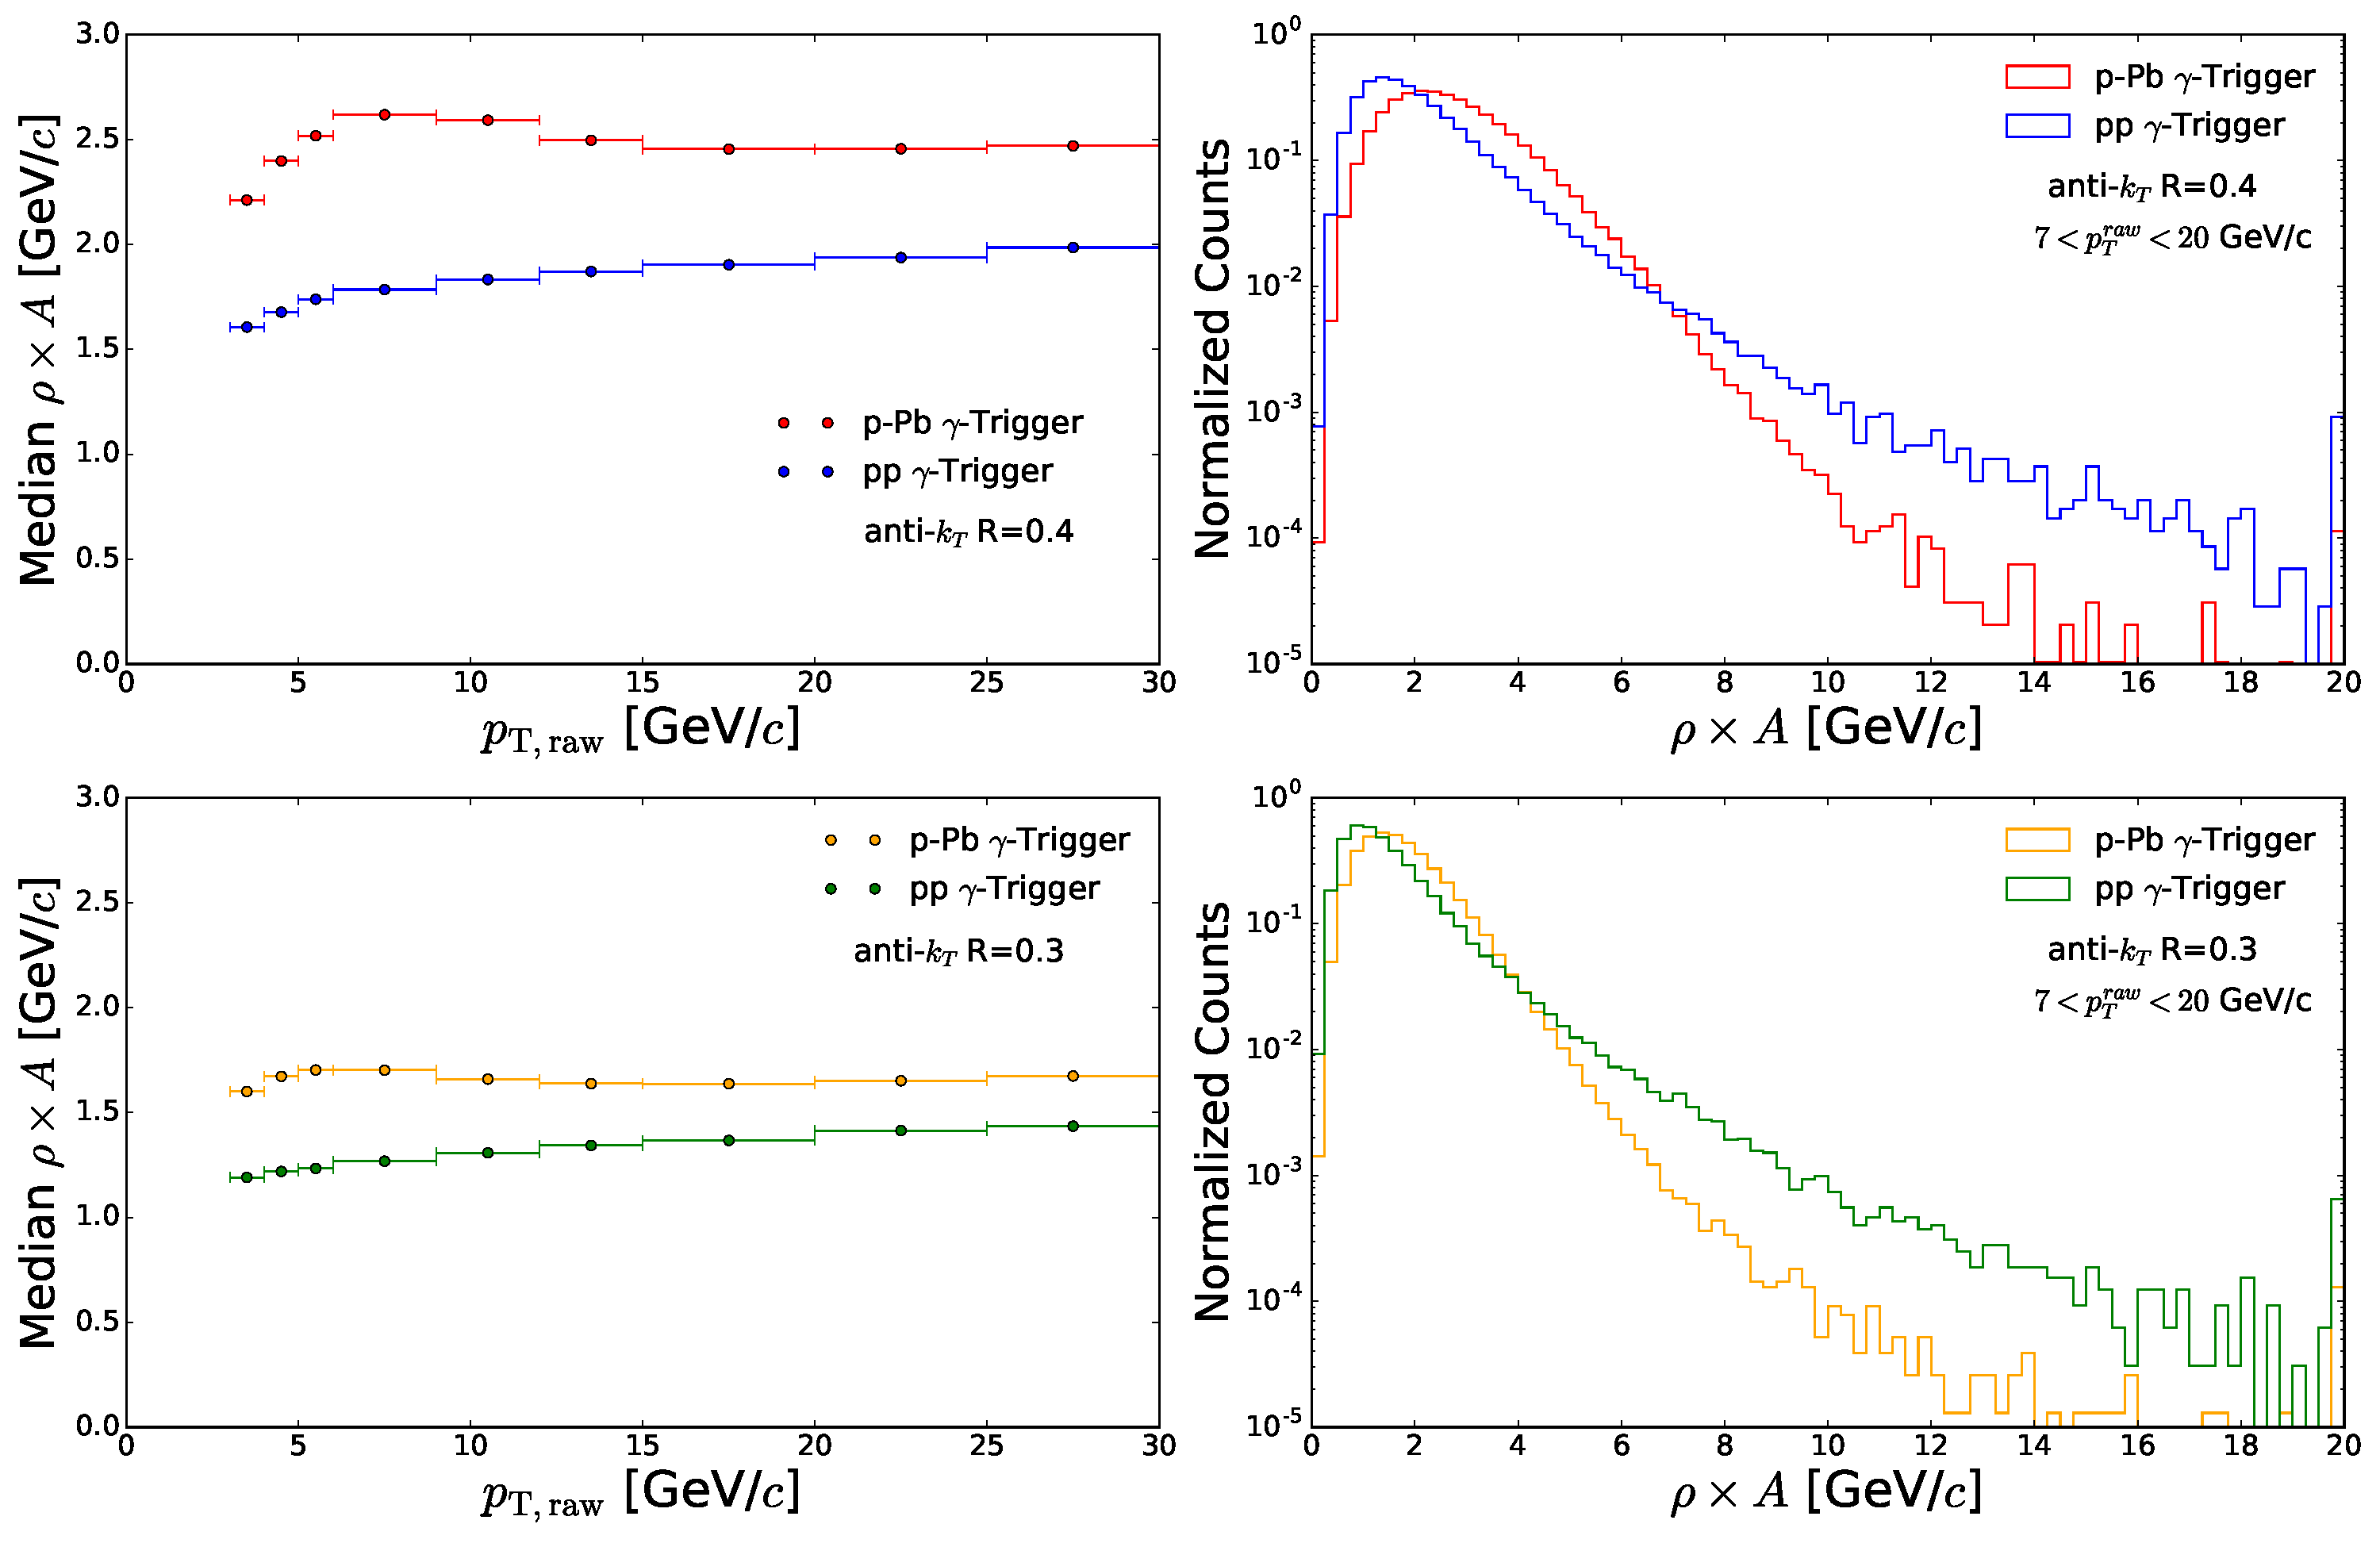
\includegraphics[width=0.99\textwidth]{JetReco/ppandpPb_median_AreaRho.pdf}
%	\caption{The average amount of UE-subtraction as a function of unsubtracted jet transverse momentum for photon-triggered events in pp and p-Pb data is shown on the left column for reconstructed jets of R = 0.3 and 0.4. The distribution of how much is UE-subtracted from jets with unsubtracted jet transverse momentum greater than {7 \GeVc} for photon-triggered events in pp and p-Pb data is shown on the right column for reconstructed jets of R = 0.3 and 0.4.}
%	\label{fig:ppandpPb_mean_RhoA}
%\end{figure}

%A recent study of of charged-jets cross-section at 7 TeV pp collisions~\cite{
%Acharya:2018eat} estimated that Multi Parton Interactions (MPIs) contribute about 50$\%$ of the cross-section for 5 $<\pt^{\mathrm{jet}}<$ 10 \GeVc~and about 20$\%$ for the range $\pt^{\mathrm{jet}}>$ 10 \GeVc. 

%This method requires the introduction of the jet area. According to the \textsc{FastJet} manual~\cite{Cacciari:2011ma}: \begin{quotation} {\it Jet areas provide a measure of the surface in the $y$-$\varphi$ plane over which a jet extends, or, equivalently, a measure of a jet’s susceptibility to soft contamination. Since a jet is made up of only a finite number of particles, one needs a specific definition in order to make its area an unambiguous concept.}\end{quotation} 

%The Voronoi~\footnote{The method used is the following fastjet::VoronoiAreaSpec \url{http://www.fastjet.fr/repo/doxygen-2.4.5/classfastjet_1_1VoronoiAreaSpec.html} }
%diagram associates each point in the $(\eta,
%\phi)$-plane with a unique track that is its nearest-neighbor by the
%Euclidean distance $\Delta R = \sqrt{\Delta\eta^2 + \Delta\phi^2}$.
%This particular choice (Euclidean Voronoi diagram) satisfies the conditions that:
%\begin{itemize}
%\item Each track resides inside the area associated with it;
%\item The sum over all areas associated with the tracks is unitary,
%  i.e.\ $3.6\pi$ for the ALICE tracking.
%\end{itemize}

%The boundary condition of the ALICE tracking at $\lvert\eta\rvert =
%0.9$ is treated as if no polygon may extend beyond, and is implemented
%using two ``mirror events'' where the particles are reflected by
%\begin{equation}
%  \eta \mapsto \pm 1.8 \mp \eta
%\end{equation}
%The cyclic boundary condition at $\lvert\phi\rvert = \pi$ is
%implemented by repeating the event with
%\begin{equation}
%  \phi \mapsto \phi \pm 2\pi
%\end{equation}
%(therefore nine copies of the same event occur during the construction
%of the Voronoi diagram).

%The empirical median function $\mathrm{med}$ is the Harrell--Davis quantile
%estimator $Q_p$ with $p =
%\frac{1}{2}$ (as opposed to the na\"{i}ve, inverse empirical
%cumulative distribution function method denoted $T_p$ therein). Note
%that unlike other definitions involving a truncated area forced to
%$\le \pi R^2$, the aforementioned properties of the Voronoi cells
%guarantee that all sparse areas are counted. This avoids the need of an ad-hoc correction factor, as used in Ref.~\cite{Adam:2015hoa}. Note that for the $k_{\mathrm{T}}$ algorithm, which is the one used for the UE estimation, the Voronoi area of a jet coincides with its ``passive area"~\cite{Cacciari:2011ma}, which is another standard \textsc{FastJet} method that has been used before by the ALICE Collaboration. 


\subsection{UE correction to isolation variable}
For each event and cluster, we subtract the underlying event using the measured charged-particle density $\rho$ that is calculated event-by-event as described in Section~\ref{sec:UEsubtraction}:
\begin{equation}
\iso = \iso^{\mathrm{raw}} - \rho\times\pi(0.4)^{2}.
\end{equation}
Thus, the average subtraction for the isolation cone of {$R=0.4$} is about {$1.6$ \GeVc} and {$0.8$ \GeVc} for \pPb~and pp collisions, with a standard deviation of {0.9 \GeVc} and {0.4 \GeVc}, respectively.  

Figure~\ref{fig:iso_ue} shows the isolation distribution before and after underlying event subtraction for \pPb~and pp collisions. The distributions have a positive tail that decreases exponentially; this is expected as this observable effectively measures multi-jet production. The difference between the \pPb~and pp distribution at low $\iso$ values can be attributed to the effect of enhanced soft-particle production in \pPb~collisions. The underlying event subtraction modifies the isolation distribution only slightly. After subtraction, the distributions show a negative tail, which arises from a over-subtraction of the underlying event due to region-to-region fluctuations. In both cases, this tail falls by more than three orders of magnitude by $\iso=-3$ \GeVc, indicating that over-subtraction is a small effect.   

\begin{figure}[h]
\center
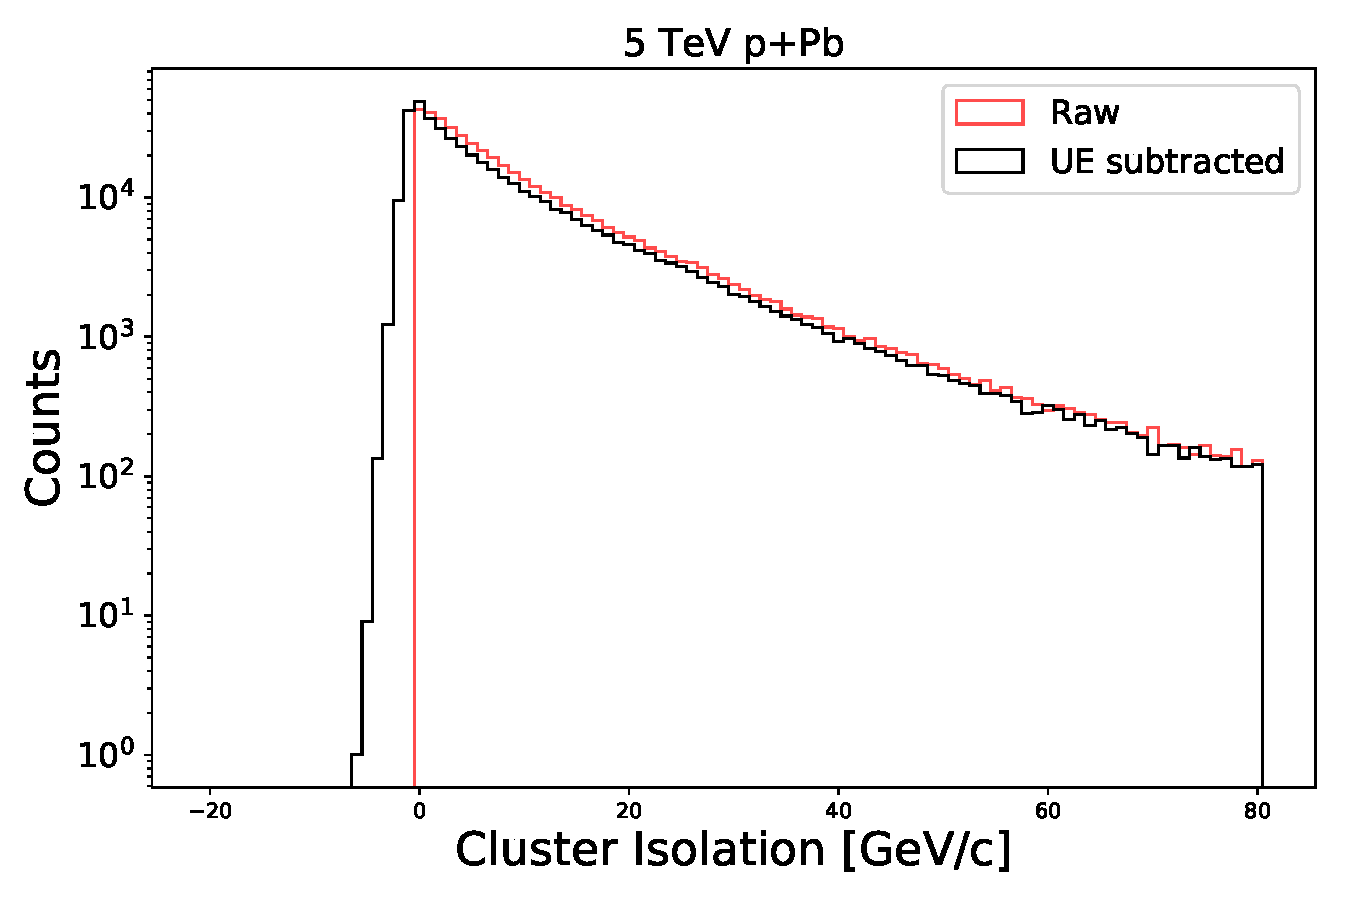
\includegraphics[width=0.49\textwidth]{Isolation/IsolationWithUESubtraction_Skimmed_13def_root}
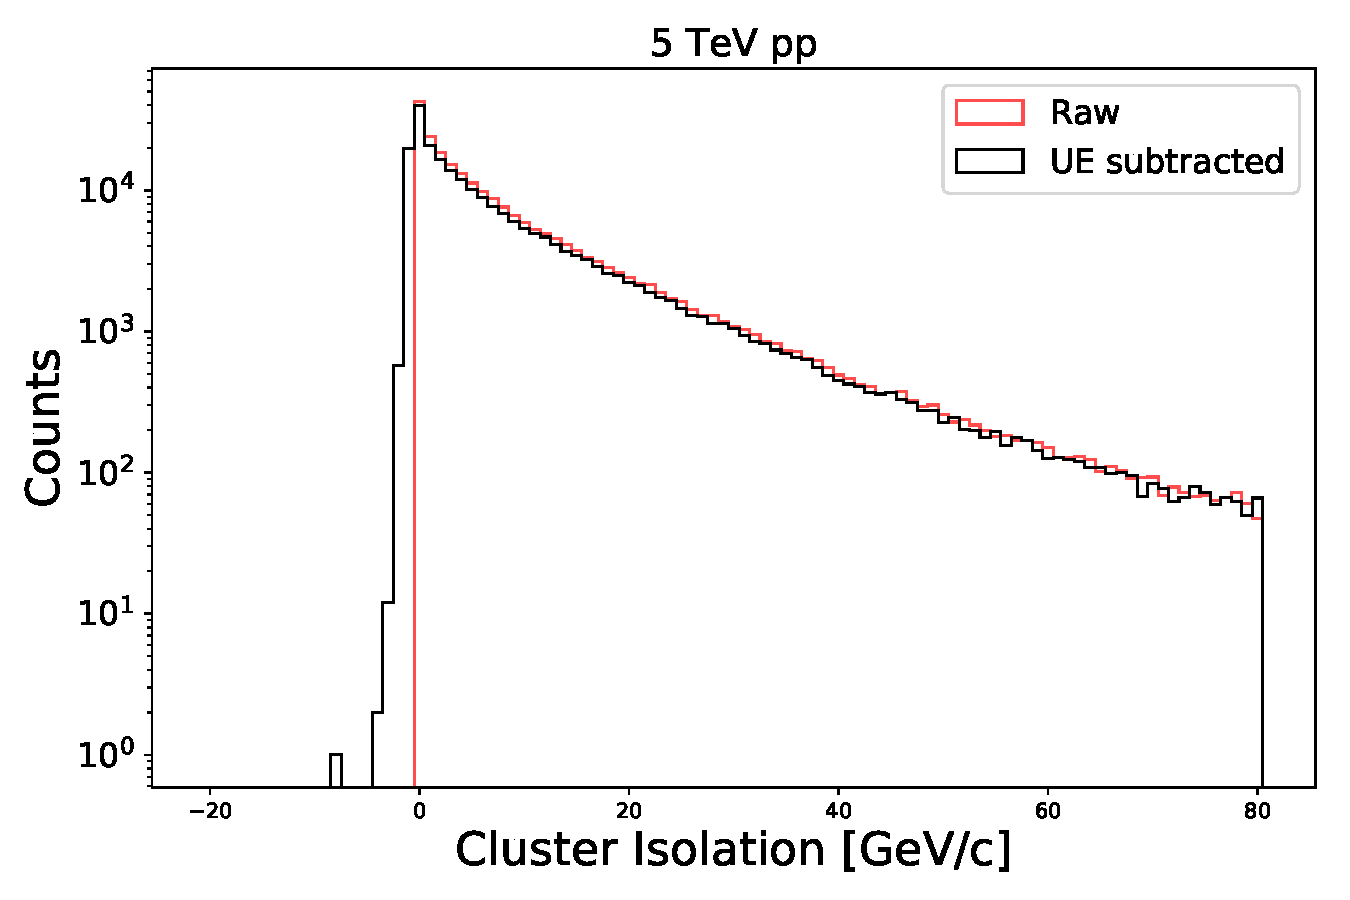
\includegraphics[width=0.49\textwidth]{Isolation/IsolationWithUESubtraction_Skimmed_17q_root}
\caption{Cluster isolation before and after underlying event subtraction in \pPb~(left panel) and pp (right panel) collisions.}
\label{fig:iso_ue}
\end{figure}

Figure~\ref{MC_Isolation} shows the distribution of cluster isolation after UE subtraction for photon-jet and dijet simulations of \pPb~data (see Table~\ref{tab:MCsamples}). As expected, the distributions are rather different: whereas the dijet simulation shows a prominent exponential tail at large $\iso$ values, the photon-jet simulation shows a Gaussian-like shape that is mostly symmetrical except for a very small fraction of events that have large $\iso$ values. In both cases, the negative tail falls rather sharply, which is expected as it arises from region-to-region fluctuations of the UE that are independent of the hard-process involved. 

\begin{figure}[h]
\center
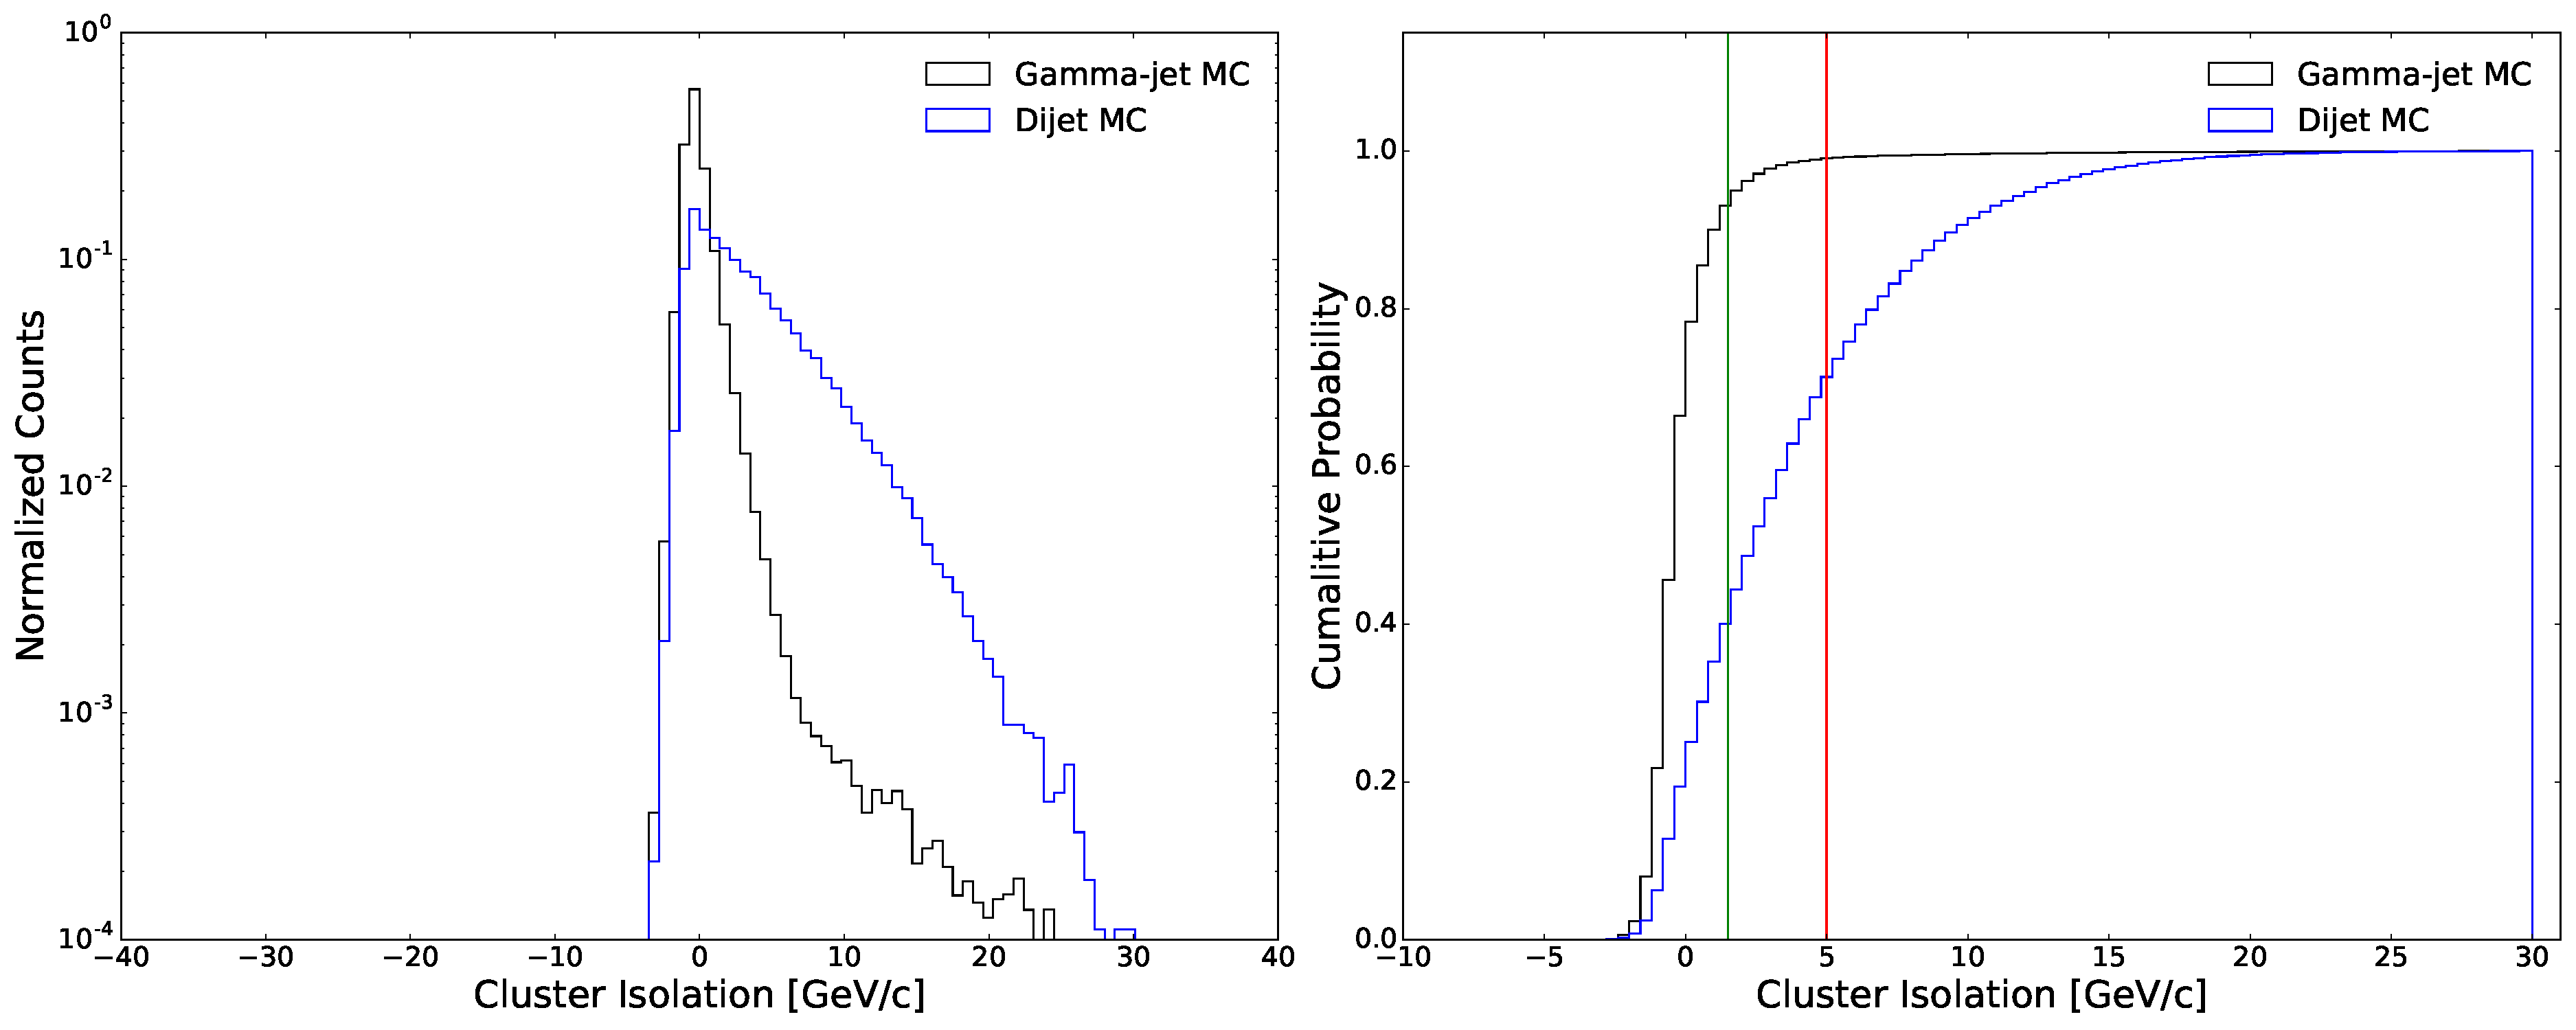
\includegraphics[width=1.0\textwidth]{Purity/Isolation_MC_pPb.pdf}
\caption{Isolation distribution of clusters that pass our selection in \pPb~photon-jet and dijet simulations, and corresponding cumulative distribution. Two vertical lines at $\iso=$ 1.5 \GeVc~(green) and $\iso=$ 5.0 \GeVc~are shown in the right panel for reference.}
\label{MC_Isolation}
\end{figure}

For the purposes of template fitting, we also need to define a sideband that is dominated by background. For this we note that only about 1$\%$ of prompt photons of the photon-jet simulation have {$\iso>$ 5 \GeVc}. Given that the cross-section for prompt photons is about two orders of magnitude smaller than the background, this region is overwhelmingly dominated by background.   
The cumulative distributions (Figure~\ref{MC_Isolation}, right panel) show that a {$\iso<$ 1.5 \GeVc} selection keeps about 90$\%$ of the signal and rejects about 60$\%$ of the background. We use this relatively loose photon isolation criteria to reduce the dependence of the results on the details of the simulation of the detector noise, tracking resolution, and the underlying event. 

This isolation cut of {$\iso<$ 1.5 \GeVc} is used in conjunction with the shower-shape cut to complete our isolated-photon selection or ``$\gammaiso$ selection''. We call ``$\gammaiso$-candidates'' the clusters that pass our isolated photon selection because it still leaves a significant fraction of background (about 40$\%$ of the cross section, as just shown). 

The main background present in our $\gammaiso$ selection is from multi-jet events where one jet typically contains a $\pi^{0}$ or $\eta$, which carries most of the jet energy, and is misidentified  as a photon because it decays into a photon pair that is collinear with respect to the EMCal cell granularity. Other sources of background arise from charged-to-neutral fluctuations of jet fragmentation that leads to low observable $\iso$ (that considers only charged-particles). 

This creates the need to measure the purity of our $\gammaiso$-candidate selection, which is described in Section~\ref{sec:purity}. 

%\subsection{Isolation efficiency}
%The isolation efficiency is ratio of the numbers of photons which pass our isolation %criteria and the rest of the cluster selection to the total number of clusters that pass the cluster selection:

%\begin{equation}
%\epsilon(\pt^{\mathrm{reco}}) = \frac{N^{\mathrm{cluster cuts + ISO cut}}(\pt^{\mathrm{reco}})}{N^{\mathrm{cluster cuts}}(\pt^{\mathrm{reco}})}.
%\end{equation}

%The cluster selection was discussed in Section~\ref{sec:clusterselection} and summarized in Table~\ref{tab:photonCutFlow}. The resulting efficiency is shown as a function of cluster \pt~in Figure~\ref{fig:isoEff}.

%The isolation efficiency is shown in Figure~\ref{fig:isoEff}. No strong dependence on $\pt$ is observed, and on average the efficiency is about 93$\%$ and 91$\%$ for pp and \pPb~ photon+jet simulated data respectively.

%We show this for illustration purposes only, because we present results normalized to the number of reconstructed photons that are, to first order, insensitive to efficiency corrections. 
%\begin{figure}[h]
%\centering
%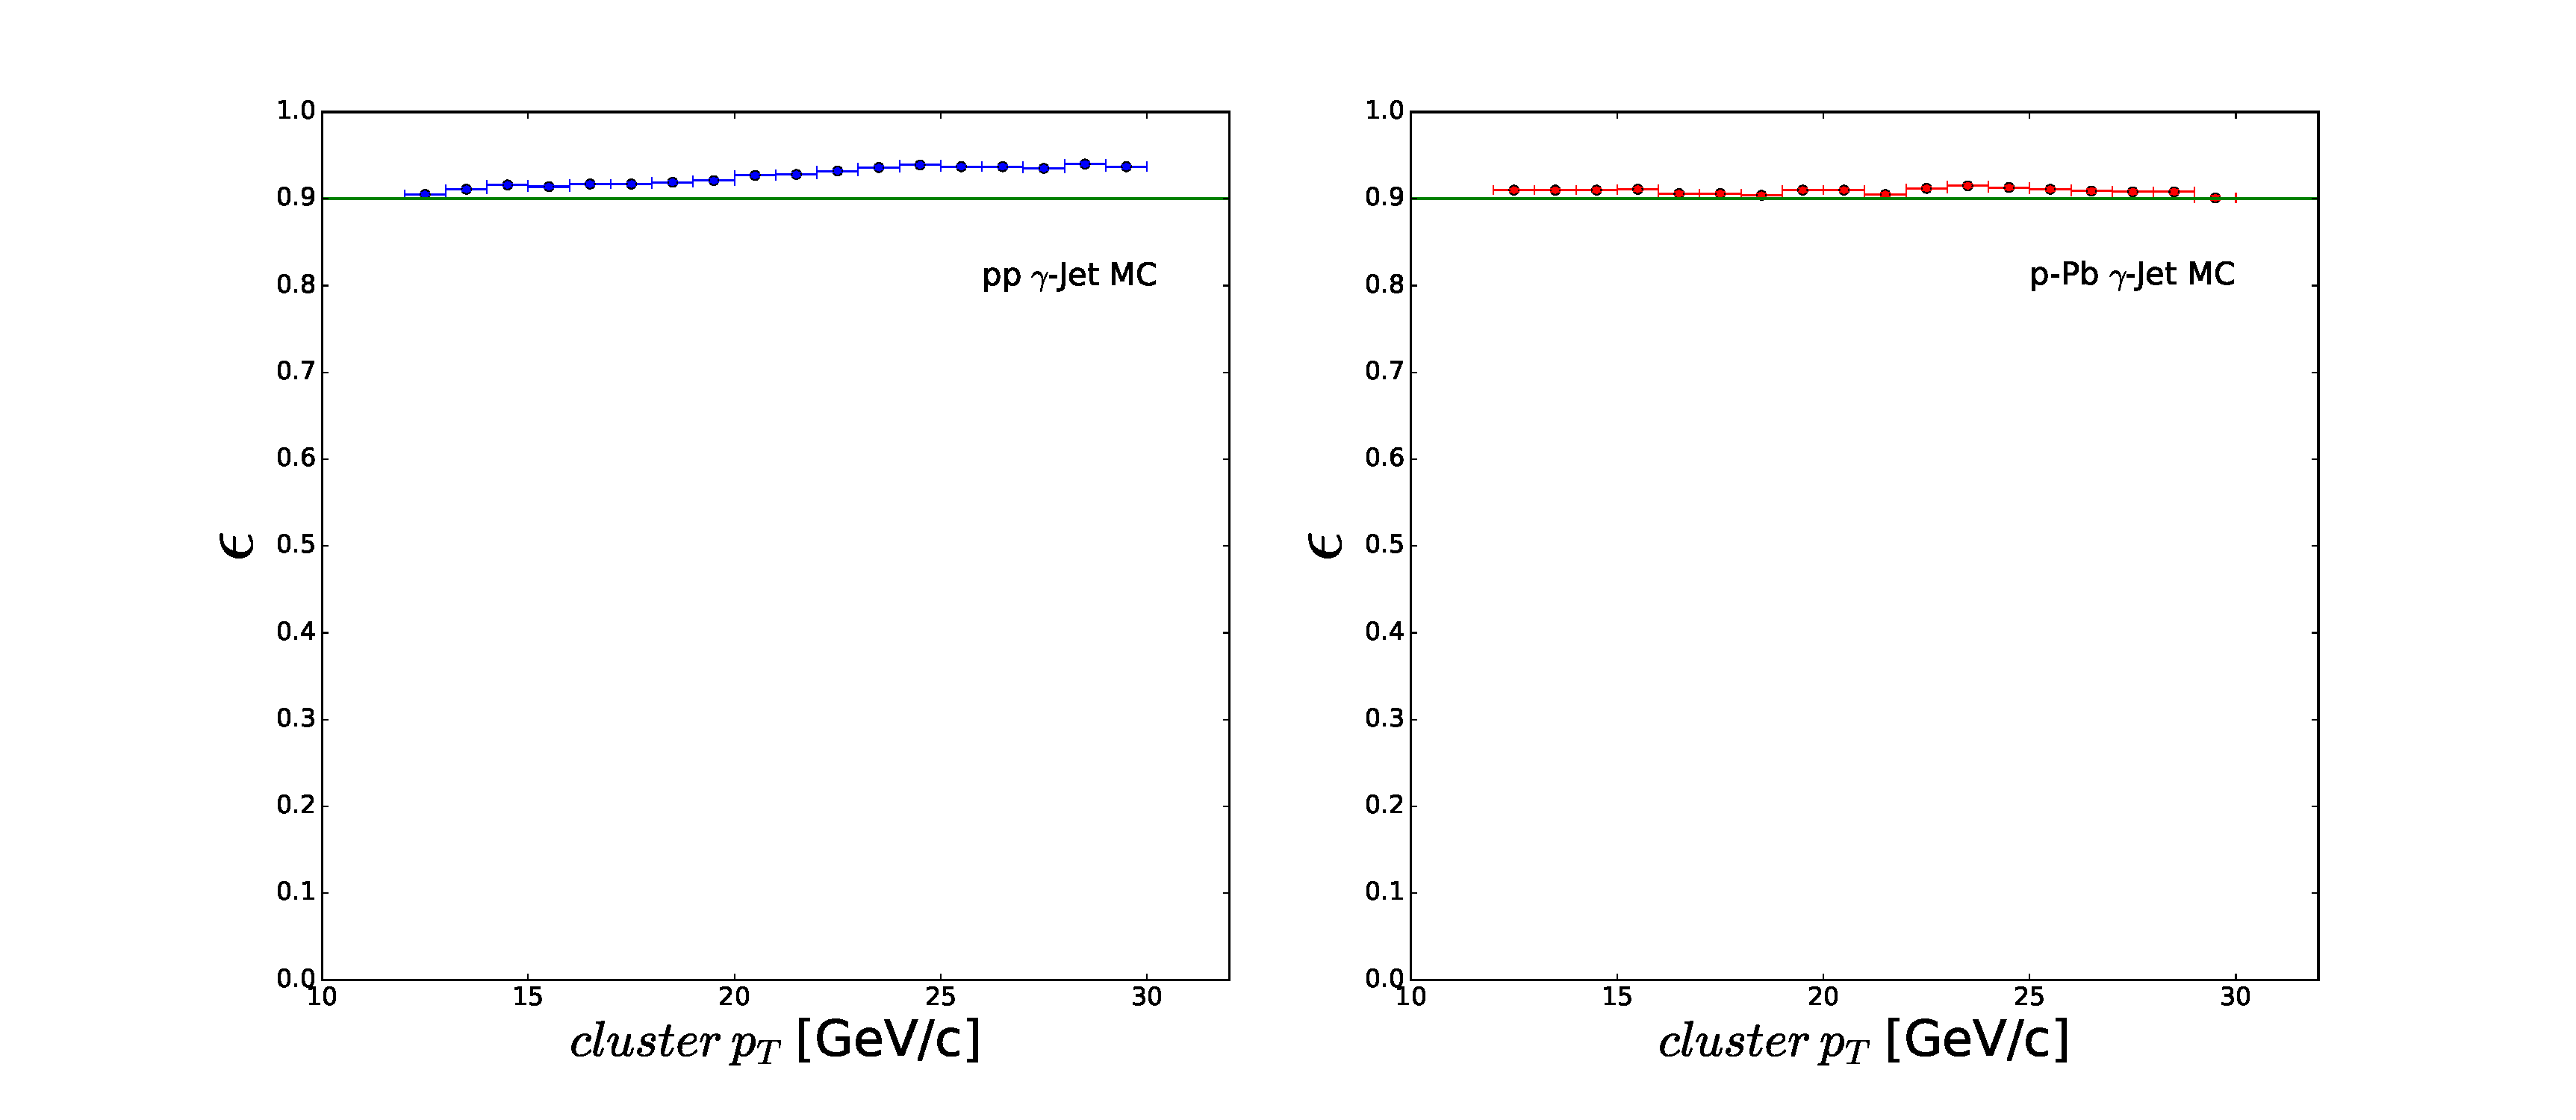
\includegraphics[width=1.0\textwidth]{EfficiencyAppendix/MC_IsoEff.pdf}
%\caption{Efficiency of isolation cut obtained from a pp and \pPb~ photon+jet simulation. A horizontal green line is placed at $\epsilon$ = 0.9 for reference. The error bars represent statistical uncertainties only.}
%\label{fig:isoEff}
%\end{figure}

%%%[still need to think about this correlation plot. Truth iso also contains UE because Pythia simulates UE. ]
%\begin{figure}[h]
%\center
%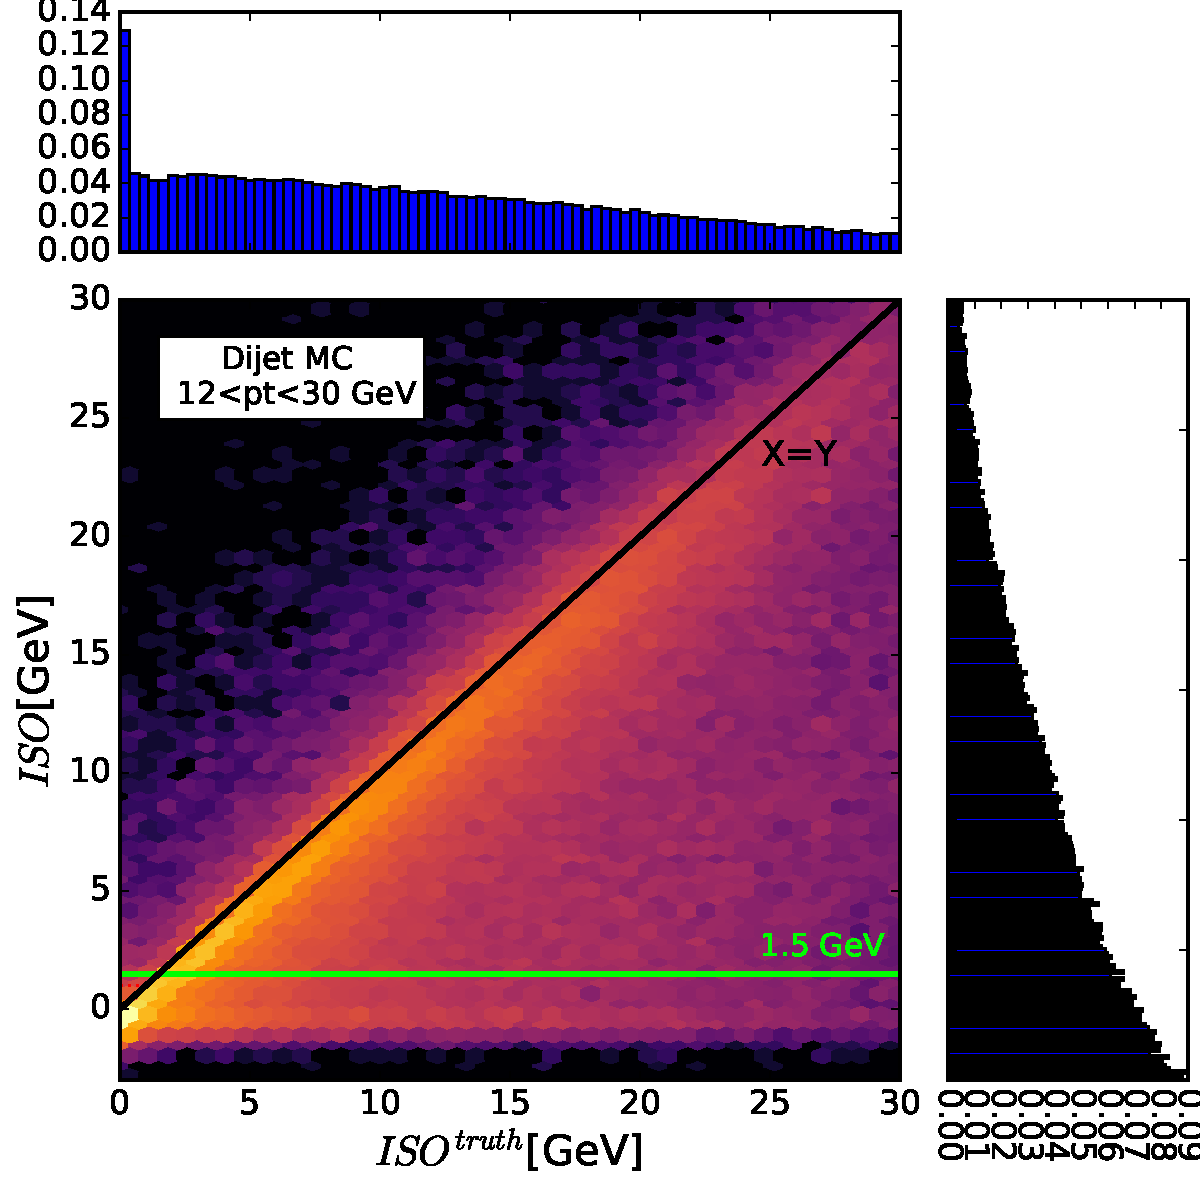
\includegraphics[height = 90mm]{Purity/pp_diject_MC.pdf}
%\caption{Correlation graph between ISO and $ISO^{truth}$ using pp Dijet MC data. The horizontal line at 1.5GeV %(green) represents the selection cut and the black is an X=Y line for reference. The correlation coefficient between ISO and $ISO^{truth}$ is found to be 70$\%$.}
%\label{pp Dijet Correlation}
%\end{figure}
